\setcounter{chapter}{3}

\chapter{不定积分}

广义地说,不定积分就是求导的“逆运算”,但由于原函数的不唯一性,我们
一般不会说它们是互逆的。

要正确和熟练地计算不定积分,必须对所有的求导公式作到“倒背如流”,
正因为如此,计算不定积分可以说是一项技术性和技巧性都比较强的工作。

\section{不定积分的概念与性质}

\subsection{原函数与不定积分}

\begin{thx}
	若在区间$I$上,$F'(x)=f(x)$,
	则称{\bf $F(x)$是$f(x)$在区间$I$上的原函数}。
\end{thx}

显然,并非所有的函数都会有原函数,例如:

{\bf 例:}证明:函数$$f(x)=\left\{\begin{array}{ll}
0\;& x\ne 0\\1\;& x=0\end{array}\right.$$在$\mathbb{R}$上不存在原函数

[证]:反证法。设$F(x)$为$f(x)$的原函数。显然,当$x\ne0$时,$F(x)=x+C(C\in\mathbb{R})$,
注意到$F(x)$必须为连续函数,故易得$F(0)=C$。

由此,
$$f(0)=F'(0)=\limx{0}\df{F(x)-F(0)}x=\limx{0}\df xx=1,$$
与已知矛盾,故假设错误,即证。\fin

参考以上的证明方法,我们可以证明{\b 所有具有第一类间断点的函数都不存在原函数}。

关于原函数的存在性,有如下的结论:

\begin{thx}
	若$f(x)$在区间$I$上连续,则必有原函数。
\end{thx}

显然,原函数具有如下的性质:

\begin{thx}
	若$F(x)$是$f(x)$在区间$I$上的原函数,则
	\begin{enumerate}
% 	  \setlength{\itemindent}{1cm}
	  \item $F(x)+C$也是$f(x)$在区间$I$上的原函数;
	  \item $f(x)$的任意两个原函数只相差一个常数。
	\end{enumerate}
\end{thx}

基于这一性质,我们给出不定积分的概念:

\begin{thx}
	函数$f(x)$在区间$I$上的全体原函数称为{\bf $f(x)$在$I$上的不定积分},
	记为
	$$\int f(x)\d x.$$
	通常情况下,若$F(x)$是$f(x)$在区间$I$上的一个原函数, 则可记
	$${\int f(x)\d x=F(x)+C},$$
	其中$C$为任意常数。
\end{thx}

{\bf 例:}不定积分表达式的多样形式
\begin{enumerate}[(1)]
  \setlength{\itemindent}{1cm}
  \item $\dint\sin x\cos x\d x=\df12\sin^2x+C$
  \item $\dint\cos x\sin x\d x=\df12\cos^2x+C$
  \item $\dint\df12\sin2x\d x=\cos2x+C$
\end{enumerate}
以上三者都属于同一个函数族,仅相差一个常数!\ps{要想判断它们是否相同,
最可靠的方法还是求导,比较其导函数是否相同}

前述关于的定义和性质用不定积分的符号来表达,可以写为

\begin{thx}
	\begin{enumerate}[(1)]
	  \item $\left(\displaystyle\int f(x)\d x\right)'=f(x)$ 
	  \item $\d\left[\displaystyle\int f(x)\d x\right]=f(x)\d x$ 
	  \item $\dint f\,'(x)\d x =f(x)+C$
	  \item $\dint \d f(x)=f(x)+C$
	\end{enumerate}
\end{thx}

\subsection{基本的不定积分公式}

从求导公式出发,逆向推导,可以得到以下的基本不定积分公式

\begin{thx}
	\begin{enumerate} [(1)]
% 	  \setlength{\itemindent}{1cm}
	  \item $(C)'=0$\hfill  {$\dint 0\d x=C$} 
	  \item $(x^a)'=ax^{a-1}$\hfill  {$\dint x^a\d x=\df{1}{a+1}x^{a+1}+C$}
	  \item $(e^x)'=e^x$\hfill  {$\dint e^x\d x=e^x+C$} 
	  \item $(a^x)'=a^x\ln a$\hfill  {$\dint a^x\d x=\df{a^x}{\ln a}+C$}
	  \item $(\ln x)'=\df 1x$\hfill  {$\dint \df 1x\d x=\ln|x|+C$}
	  \item $(\sin x)'=\cos x$\hfill  {$\dint \cos x\d x=\sin x+C$} 
	  \item $(\cos x)'=\sin x$\hfill  {$\dint \sin x\d x=-\cos x+C$}
	  \item $(\tan x)'=\sec^2 x$\hfill  {$\dint \sec^2 x\d x=\tan x+C$} 
	  \item $(\cot x)'=-\csc^2 x$\hfill  {$\dint \csc^2 x\d x=-\cot x+C$}
	  \item $(\sec x)'=\sec x\tan x$\hfill $\dint\sec x\tan x\d x=\sec x+C$
	  \item $(\csc x)'=-\csc x\cot x$\hfill $\dint\csc x\cot x\d x=-\csc x+C$
	  \item $(\arcsin x)'=\df{1}{\sqrt{1-x^2}}$ \hfill  
	  {$\dint{\df{1}{\sqrt{1-x^2}}}\d x=\arcsin x+C$} 
	  \item $(\arctan x)'=\df{1}{1+x^2}$ \hfill 
	  {$\dint \df{1}{1+x^2}\d x=\arctan x+C$}
	  \item $(\cosh x)'=\sinh x$ \hfill $\dint\sinh x\d x=\cosh x+C$
	  \item $(\sinh x)'=\cosh x$ \hfill $\dint\cosh x\d x=\sinh x+C$
	\end{enumerate}
\end{thx}

{\bf 注:}$x>0$时,$(\ln x)'=\df 1x$,所以$\dint\df{\d x}x=\ln x+C$,
$x<0$时,$(\ln(-x))'=\df1x$,所以$\dint\df{\d x}x=\ln(-x)+C$

{\bf 例:}计算不定积分
\begin{enumerate}[(1)]
  \setlength{\itemindent}{1cm}
  \item $\dint x^2\sqrt{x}\d x$ 
  \item $\dint \df{1}{x\sqrt[3]{x}}\d x$ 
  \item $\dint \df{4^x}{9^x}\d x$ 
  \item $\dint 2^x3^{2x}5^{3x}\d x$
\end{enumerate}

\subsection{不定积分的基本性质}

\begin{thx}
	{\bf 线性性:}设函数$f(x),g(x)$的原函数存在,则
	$$\int[\alpha f(x)+\beta g(x)]\d x
	=\alpha\int f(x)\d x+\beta\int g(x)\d x,$$
	其中$\alpha,\beta$为任意常数。
\end{thx}

{\bf 例:}计算不定积分
\begin{enumerate}[(1)]
  \setlength{\itemindent}{1cm}
  \item $\dint (4x^3-2x^2+5x+3)\d x$
  \item $\dint(1-2x)^2\sqrt x\d x$
  \item $\dint\df{(x-\sqrt x)(1+\sqrt x)}{\sqrt[3]x}\d x$
  \item $\dint\df{\d x}{\sin^2x\cos^2x}$
  \item $\dint(10^x+3\sin x+\sqrt x)\d x$
  \item $\dint\sum\limits_{k=0}^na_kx^k\d x$
  \item $\dint (x^2+1)^2\d x$ 
  \item $\dint\df{(x+1)^3}{x^2}\d x$ 
  \item $\dint\df{1-x^2}{x^2(1+x^2)}\d x$
  \item $\dint\df{2x^4+x^2+3}{x^2+1}\d x$
  \item $\dint \df{x^4}{1+x^2}\d x$ 
  \item $\dint\df{1}{1+\cos 2x}\d x$ 
  \item $\dint\tan^2 x\d x$
\end{enumerate}

\begin{ext}
	{\bf 课后作业}
	\begin{enumerate}
	  \item 同济教材习题4-1:2,5,6
	  \item 同济教材总习题四:3
	\end{enumerate}
\end{ext}

\section{换元积分法}

仅仅使用基本的积分公式以及不定积分的线性性,能够计算的不定积分类型还是
非常有限的。本节介绍的还原积分法,是计算不定积分时最为常用和基本的方法,
它的基本思想直接来源于对复合函数的求导法则(链式法则)的逆向思维。

\subsection{第一换元法}

假设$F(x)$为$f(x)$的任意一个原函数,考虑$F(x)$与另一个函数$\varphi(x)$
复合函数,由复合函数求导法则,有
$$[F(\varphi(x))]'=F'(\varphi(x))\varphi'(x),$$
对上式两边同时取不定积分,利用基本的
$$\dint F'(\varphi(x))\varphi'(x)
=\dint[F(\varphi(x))]'\d x=F(\varphi(x))+C=F(u)+C
=\left[\dint f(u)\d u\right]_{u=\varphi(x)}.
$$
从而我们得到:
\begin{thx}
	{\bf 积分第一换元法:}设$f(u)$具有原函数,$u=\varphi(x)$可导,则
	$$\dint f[\varphi(x)]\varphi'(x)\d x=\left[\dint f(u)
	\d u\right]_{u=\varphi(x)}$$
\end{thx}

理解积分的第一换元法,也可以从微分运算的角度出发
$$F'(\varphi(x))\varphi'(x)\d x
=F'(\varphi(x))\d\varphi(x)
=\d F(\varphi(x))=\left.\d F(u)\right|_{u=\varphi(x)}.$$
两边同时计算不定积分,即得前述的公式。

从公式的表达上看,积分第一换元法似乎让人不得要领,但在实际运用时,
确实非常简单和方便的,我们通常将其看成是一个将微分运算符号$\d$
前的所有函数部分,都(利用基本的求导/积分公式)“移到”$\d$之后
的过程,因此我们常常也将积分第一换元法称为{\kaishu “凑微分法”}。

{\bf 例:}计算下列不定积分
\begin{enumerate}[(1)]
  \setlength{\itemindent}{1cm}
  \item $\dint\cos 2x\d x$ 
  \item $\dint\df 1{3+2x}\d x$
  \item $\dint\df{\d x}{x^2-a^2}$
  \item $\dint 2xe^{x^2}\d x$ 
  \item $\dint\df{x^2}{(x+2)^3}\d x\xlongequal{x+2=t}\ldots$ 
  \item $\dint\df 1{a^2+x^2}\d x=\df1a\dint\df1{1+(x/a)^2}\d\df xa=\ldots$ 
  \item $\dint\df 1{\sqrt{a^2-x^2}}\d x=\dint\df1{\sqrt{1-(x/a)^2}}\d\df
  xa=\ldots$
%   \hfill(令$t=\sqrt{a^2-x^2}$没有直接的效果,但可令$t=\sqrt{\df{a+x}{a-x}}$)
  \item $\dint \df 1{x(1+2\ln x)}\d x$ 
  \item $\dint\df {e^{3\sqrt x}}{\sqrt x}\d x=2\dint e^{\sqrt x}\d\sqrt x=\ldots$ 
  \item $\dint \sin^3x\d x=-\dint(1-\cos^2x)\d\cos x=\ldots$ 
  \item $\dint \sin^2x\cos^4x\d x=\df18\dint\sin^22x(1+\cos2x)\d x
  =\df18\dint\sin^22x\d x+\df1{16}\dint\sin^2x\d\sin^2x=\ldots$ 
  \item $\dint\sec^6x\d x=\dint(1+\tan^2 x)^2\d\tan x=\ldots$ 
  \item $\dint\sec x\d x=\dint\df{\cos x\d x}{1-\sin^2x}
  \xlongequal{t=\sin x}\dint\df{\d t}{1-t^2}=\ldots$
%   \hfill($\dint\df{\sec x(\sec x+\tan x)}{(\sec x+\tan
%   x)}\d x=\ln|\sec x+\tan x|+C$)
\end{enumerate}

{\bf 注:}{\b 换元的基本原则:优先替换不好处理的部分,即{\it “看谁不顺眼就换谁”!}}

\subsection{第二换元法}

积分第一换元法利用变换$u=\varphi(x)$,将积分$\dint f(\varphi(x))\d x$
化为积分$\dint f(u)\d u$,第二换元法则尝试相反的方向,即利用某个变换$x=\psi(t)$,
将积分$\dint f(x)\d x$化为$\dint f(\psi(t))\psi'(t)\d t$。

\begin{thx}
	{\bf 积分第二换元法:}
	设$x=\psi(t)$可导且可逆,$f(\psi(t))\psi'(t)$
	存在原函数,则
	$$\dint f(x)\d x=\dint f(\psi(t))\psi'(t)\d t$$
\end{thx}

{\bf 例:}计算下列不定积分
\begin{enumerate}[(1)]
  \setlength{\itemindent}{1cm}
  \item $\dint \sqrt{a^2-x^2}\d x\xlongequal{x=|a|\sin t}\dint a^2\cos^2t\d t
  =\df{a^2}2\dint(1+\cos2t)\d t=\ldots$ 
  \item $\dint\df{\d x}{\sqrt{x^2+a^2}}\xlongequal{x=|a|\tan t}
  \dint\sec t\d t=\ldots$
  \item $\dint\df{\d x}{(x^2+a^2)^2}\xlongequal{x=|a|\tan t}
  \df1{|a|^3}\dint\cos^3t\d t=\ldots$
  \item $\dint\df{\d x}{\sqrt{x^2-a^2}}\xlongequal{x=|a|\sec t}
  \dint\tan t\d t=\ldots$ 
  \item $\dint \df{1}{1+\sqrt x}\d x\xlongequal{\sqrt x=t}\ldots$ 
  \item $\dint\df{\d x}{1+\sqrt[3]{x+2}}\xlongequal{x+2=t^3}\ldots$ 
  \item $\dint\df{\sqrt{a^2-x^2}}{x^4}\d x\xlongequal{x=|a|\sin t}\ldots$
\end{enumerate}

不论是第一换元法,还是第二换元法,其核心都是利用变量的代换,改变被积函数的形态,
从而达到接近或转化为基本的不定积分的目的,从这个意义上说,二者没有什么不同。当然,
根据被积函数结构的特点,也会有一些常用的变换技巧,具体我们将在本章最后一节中集中讨论。

\begin{ext}
	{\bf 计算下列不定积分}
	
	\begin{enumerate}
	  \item $\dint\cos2x\sin x\d x$
	  \item $\dint\df1{4+x^2}\d x$
	  \item $\dint\df{x+2}{x^2+2}\d x$
	  \item $\dint\sec^4x\d x$
	  \item $\dint\sqrt{a^2+x^2}\d x$
	  \item $\dint x^3\sqrt{a^2+x^2}\d x$
	  \item $\dint\df{\sin(2+\sqrt x)}{\sqrt x}\d x$
	  \item $\dint\df1{1-x^2}\d x$
	  \item $\dint\df1{x(1-x^2)}\d x$
	  \item $\dint\sin^2x\cos^3x\d x$
	  \item $\dint\df1{x(1+\sqrt x)}\d x$
	  \item $\dint\df1{1-\sqrt[3]{x-1}}\d x$
	  \item $\dint\df{x}{x^2+x+1}\d x$
	  \item $\dint\df{x^2}{x^2+x+1}\d x$
	  \item $\dint\df{x}{(x-2)(x-3)}\d x$
	  \item $\dint\df1{x^2+x+1}\d x$
	  \item $\dint\df{\sin(x+a)}{\sin x}\d x$
	  \item $\dint\df{\sin x}{\sin(x+a)}\d x$
	  \item $\dint\df{\d x}{e^x-1}$
	  \item $\dint\sin4x\cos6x\d x$
	\end{enumerate}
\end{ext}

\section{分部积分法}

注意到对可导函数$u,v$,有
$$\d uv=u\d v+v\d u\quad\Leftrightarrow\quad 
u\d v=\d uv-v\d u,$$
后一式两边同时不定积分,可得
\begin{thx}
	{\bf 分部积分公式:}
	$${\b \dint u\d v=uv-\dint v\d u}$$
\end{thx}

{\bf 例:}计算下列不定积分
\begin{enumerate}[(1)]
  \setlength{\itemindent}{1cm}
  \item $\dint x\cos x\d x$ 
  \item $\dint xe^x\d x$ 
  \item $\dint x^2e^x\d x$ 
  \item $\dint\ln x\d x$
  \item $\dint x\ln x\d x$ 
  \item $\dint x\arctan x\d x$ 
  \item $\dint e^x\sin x\d x$
  \item $\dint\csc^4x\d x$\\
  $$I=-\cot x\csc^2x+\dint\cot x\d(\csc^2x)=-\cot x\csc^2x-2I-2\cot x$$
  \item $\dint x\tan x\sec^2x\d x$
  $$I=\df12x\sec^2x-\df12\dint\sec^2\d x=\df12(x\sec^2x-\tan x)+C$$
  下面的解法错在哪里?令$x=\pi-t$\ps{求导验证结果不正确!}{\b
  \begin{align}
  I&=\dint\df{(\pi-t)\sin t}{\cos^3t}\d t=\pi\dint\df{\sin t}{\cos^3t}\d t
  -\dint\df{t\sin t}{\cos^3t}\d t\notag\\
  &=\pi\dint\d\left(\df1{2\cos^2t}\right)-I=\df{\pi}2\sec^2t-I\notag
  \end{align}
  故$I=\df{\pi}4\sec^2x+C$}
  \ps{$\dint\df{t\sin t}{\cos^3t}\d t\ne I$}
  \item $\dint\df{x\ln x}{(1+x^2)^2}\d x$
  \item $\dint\df{x\arctan x}{(1+x^2)^2}\d x$
\end{enumerate}

{\bf 注:}{\b {\it “{反对}不要碰,{三指}动一动”}——处理分部积分的一个大致原则,即:
按照{\it {“三指幂对反”}}的次序将被积函数中对应的部分放到微分符号后面}

\begin{ext}
	{\bf 计算下列不定积分}
	
	\begin{enumerate}
	  \item $\dint x^2\ln x\d x$
	  \item $\dint x\cos^2x\d x$
	  \item $\dint e^{ax}\cos bx\d x$
	  \item $\dint x\arcsin x\d x$
	  \item $\dint\df1{(1+x^2)^2}\d x$
	  \item $\dint\sqrt{1-x^2}\arcsin x\d x$
	  \item $\dint\df{xe^x}{(e^x+1)^2}\d x$
	  \item $\dint\ln^2(x+\sqrt{1+x^2})\d x$
	  \item $\dint\df{x+\sin x}{1+\cos x}\d x$
	  \item $\dint\arctan\sqrt{x}\d x$
	\end{enumerate}
\end{ext}

\section{有理函数的积分}

\subsection{有理函数的积分法}

有理函数也叫{\it 有理分式函数},是两个多项式函数相除的商。

\begin{thx}
	{\bf 有理函数(有理分式):}$$f(x)=\df{P(x)}{Q(x)}$$
	其中$P(x),Q(x)$均为多项式函数 ,若$P(x)$的次数小于$Q(x)$的次数,
	称该函数为{\it 真分式} 。
\end{thx}

在我们所接触的积分问题中,很多时候被积函数都可以通过换元化为
有理函数,因此,研究有理函数的积分就具有了非常广泛而普遍的意义。

另一方面,通过研究发现,所有的有理函数都是存在不定积分的,
求解有理函数积分的思路对于我们求解其他的积分问题可能也具有借鉴的意义。

具体来说,求解有理函数积分的核心思想是“分解”,也即将一个普通的有理函数
分解为多个常见或相对简单的函数的和,然后完成逐个积分。

\subsubsection{有理函数的分解}

利用{\b\it 多项式除法},任意不是真分式的有理函数都可以表示成
一个多项式与一个真分式的和,例如:
$$\df{2x^4+x^2+3}{x^2+1}=2x^2-1+\df{4}{x^2+1}$$
$$\df{x^3+x^2-1}{x-1}=x^2+2x+2+\df1{x-1}$$
具体的除法过程如下,类似于小学学习过的竖式除法
\begin{center}
	\polylongdiv{x^3+x^2-1}{x-1}
\end{center}

显然多项式函数的不定积分是非常容易的,下面集中讨论真分式的积分问题。

\subsubsection{真分式的分解}

\begin{thx}
	{\bf 有理真分式的分解:}若多项式函数$Q(x)$具有如下的分解
	$$Q(x)=Q_1(x)Q_2(x),$$
	其中$Q_1(x)$和$Q_2(x)$没有公因式,则真分式$\df{P(x)}{Q(x)}$
	必可分解为如下的形式
	$$\df{P(x)}{Q(x)}=\df{P_1(x)}{Q_1(x)}+\df{P_2(x)}{Q_2(x)},$$
	其中等式右端的两个有理函数均为真分式。
\end{thx}
利用以上的性质,任何有理真分式最终都可以化成形如
$\df{P_1(x)}{(x-a)^k},\df{P_2(x)}{(x^2+px+q)^l}$(其中$(p^2-4q<0)$,
$P_1(x)$和$P_2(x)$的次数分别小于$k$和$2l$次)的真分式的和的形式。
再已知分母的分解的前提下,利用{\it 待定系数法}很容易完成真分式的分解。

{\bf 例:}将有理函数$\df{x+2}{x^2-5x+6}$分解为真分式的和。

[解]:注意到$x^2-5x+6=(x-2)(x-3)$,故可设
$$\df{x+2}{x^2-5x+6}=\df{A}{x-2}+\df{B}{x-3},$$
通分整理后,相除分母可得
$$x+2=(A+B)x-2A-3B,$$
从而根据多项式函数的性质({\it 两个多项式恒等,当且仅当其对应项的系数完全相同}),有
$$
	\left\{\begin{array}{l}
		A+B=1\\
		2A+3B=-2
	\end{array}\right.
	\quad\Rightarrow\quad
	\left\{\begin{array}{l}
		A=5\\
		B=-4
	\end{array}\right.
$$
故
$$x^2-5x+6=(x-2)(x-3)=\df{5}{x-2}-\df4{x-3}.$$
\fin

{\bf 例:}将有理函数$\df{x+2}{(2x+1)(x^2+x+1)}$分解为真分式的和。

[解]:设
$$\df{x+2}{(2x+1)(x^2+x+1)}
=\df{A}{2x+1}+\df{Bx+C}{x^2+x+1},$$
通分整理后可得
$$x+2=(A+2B)x^2+(A+B+2C)x+(A+C).$$
进而
$$
	\left\{\begin{array}{l}
		A+2B=0\\
		A+B+2C=1\\
		A+C=2
	\end{array}\right.
	\quad\Rightarrow\quad
	\left\{\begin{array}{l}
		A=2\\
		B=-1\\
		C=0
	\end{array}\right.
$$
故
$$\df{x+2}{(2x+1)(x^2+x+1)}
=\df{2}{2x+1}-\df1{x^2+x+1}.$$
\fin

以下继续讨论$\df{P_1(x)}{(x-a)^k}$和$\df{P_2(x)}{(x^2+px+q)^l}$的积分:

\subsubsection{求解$\dint\df{P_1(x)}{(x-a)^k}\d x$}

\begin{thx}
	\begin{itemize}
	  \item $\dint\df A{x-a}\d x=A\ln|x-a|+C$
	  \item $\dint\df{B\d x}{(x-a)^n}=\df B{(1-n)(x-a)^{n-1}}+C$
	  \item $\dint\df{Q(x)}{(x-a)^n}$,令$u=x-a$,将其化成若干个前两种形式的和
	\end{itemize}
\end{thx}

{\bf 例:}
 $\dint\df x{(x+1)^3}\d x\xlongequal{u=x+1}\dint\df{u-1}{u^3}\d u
 =\dint\df1{u^2}\d u-3\dint\df1{u^3}\d u=\ldots$
 
 {\bf 例:}
 $\dint\df{x^2}{(x-2)^3}\d x\xlongequal{u=x-2}
 \dint\df{u^2-4u+4}{u^3}\d u
 =\dint\df1u\d u-4\dint\df{\d u}{u^2}+4\dint\df{\d u}{u^3}=\ldots$

\subsubsection{求解$\dint\df{P_2(x)}{(x^2+px+q)^l}\d x$}

先考虑$l=1$的情形:

\begin{thx}
	$\dint\df{Ax+B}{x^2+px+q}\d x$
	
	令$y=x+\frac p2$,记$u=\sqrt{q-\frac{p^2}4}$,$F=B-\frac{Ap}2$,则
	\begin{align*}
		\dint\df{Ax+B}{x^2+px+q}\d x
		&=\dint\df{Ay+F}{y^2+u^2}\d y
		=A\dint\df{y}{y^2+u^2}\d y+F\dint\df1{y^2+u^2}\d y\\
		&=\df{A}{2\ln(y^2+u^2)}+\df{F}{u}\arctan\df yu+C\\
		&=\df{A}{2(x^2+px+q)}+\df{B-\frac{Ap}2}{\sqrt{q-\frac{p^2}4}}
		\arctan\df{x+\frac p2}{\sqrt{q-\frac{p^2}4}}+C
	\end{align*}
\end{thx}

{\bf 例:}$\dint\df{1}{x^2+x+1}\d x$

[解]:
\begin{align*}
	\mbox{原式}&=\dint\df1{(x+\frac12)^2+\frac34}\d x
	\xlongequal{y=x+\frac12}\df2{\sqrt3}
	\dint\df1{[\frac{2}{\sqrt3}y]^2+1}\d {\df2{\sqrt3}y}\\
	&=\df2{\sqrt3}\arctan\df2{\sqrt3}y
	=\df2{\sqrt3}\arctan\df2{\sqrt3}\left(x+\df12\right)+C.
\end{align*}
\fin

{\bf 例:}$\dint\df{x+1}{x^2+x+1}\d x$

[解]:
\begin{align*}
	\mbox{原式}&=\dint\df{(x+\frac12)+\frac12}{(x+\frac12)^2+\frac34}\d x
	=\dint\df{x+\frac12}{(x+\frac12)^2+\frac34}\d x
	+\df12\dint\df1{x^2+x+1}\d x\\
	&=\df12\dint\df1{(x+\frac12)^2+\frac34}\d\left(x+\frac12\right)^2
	+\df12\dint\df1{x^2+x+1}\d x\\
	&=\df12\dint\df1{(x+\frac12)^2+\frac34}\d\left[\left(x+\frac12\right)^2
	+\df34\right]
	+\df12\dint\df1{x^2+x+1}\d x\\
	&=\df12\ln\left[\left(x+\frac12\right)^2
	+\df34\right]+\df1{\sqrt3}\arctan\df2{\sqrt3}\left(x+\df12\right)+C\\
	&=\df12\ln(x^2+x+1)
	+\df1{\sqrt3}\arctan\df2{\sqrt3}\left(x+\df12\right)+C.
\end{align*}

\begin{shaded}
	{\bf 计算形如$\dint\df{\d x}{x^2+px+q}$的积分:}
	
	记$\Delta=p^2-4q$,
	
	(i)若$\Delta>0$,则记$x_{1,2}=\df{-p\pm\sqrt{\Delta}}2$为$x^2+px+q=0$
	的两个相异实根,于是
	\begin{align}
		\dint\df{\d x}{x^2+px+q}&=\dint\df{\d x}{(x-x_1)(x-x_2)}
		=\df1{x_1-x_2}\dint\left(\df1{x-x_1}-\df1{x-x_2}\right)\d x\notag\\
		&=\df2{\sqrt{\Delta}}\ln\left|\df{x-x_1}{x-x_2}\right|+C\notag\\
		&=\df2{\sqrt{p^2-4q}}\ln\left|\df{2x+p-\sqrt{p^2-4q}}
		{2x+p+\sqrt{p^2-4q}}\right|+C\notag
	\end{align}
	
	(ii)若$\Delta=0$,则$x=-\df p2$为$x^2+px+q=0$的二重根,从而
	$$\dint\df{\d x}{x^2+px+q}=\dint\df{\d x}{(x+p/2)^2}=-\df2{2x+p}+C$$
	
	(iii)若$\Delta<0$,令$u=x+\df p2$,记$A=\sqrt{-\Delta/4}=\df{\sqrt{4q-p^2}}2$则
	\begin{align}
		\dint\df{\d x}{x^2+px+q}&=\dint\df{\d u}{u^2+A^2}
		=\df1A\dint\df{\d(u/A)}{(u/A)^2+1}\notag\\
		&=\df1A\arctan\df uA+C=\df2{\sqrt{-\Delta}}
		\arctan\df{2x+p}{\sqrt{-\Delta}}+C\notag\\
		&=\df2{\sqrt{4q-p^2}}\arctan\df{2x+p}{\sqrt{4q-p^2}}+C\notag
	\end{align}
\end{shaded}

对于更一般的情形($l>1$),可以使用分部积分,得到如下的公式\ps{了解即可}:

\begin{thx}
	$$\dint\df{Ax+B}{(x^2+px+q)^l}\d x=
	\df A{2(1-l)(x^2+px+q)^{l-1}}+\left(B-\df{Ap}2\right)J_l,$$
	其中令$y=x+\frac p2$,记$u=\sqrt{q-\frac{p^2}4}$,则
	\begin{align*}
		J_l&=\df{y}{2u^2(l-1)(y^2+u^2)^{l-1}}+
  		\df{3-2l}{2u^2(1-l)}J_{l-1},\\
  		J_1&=\df1u\arctan\df yu+C.	
	\end{align*}
\end{thx}

{\bf 例:}计算积分:$I_2=\dint\df{\d x}{(1+x^2)^2}$


[解]:
\begin{align}
	I_2&=\dint\df{\d x}{(1+x^2)^2}
	=\dint\df{(1+x^2)-x^2}{(1+x^2)^2}\d x
	=\dint\df{\d x}{1+x^2}-\df12\dint\df{x\d x^2}{(1+x^2)^2}\notag\\
	&=\dint\df{\d x}{1+x^2}+\df12\dint x\d\df1{1+x^2}\notag
	=\dint\df{\d x}{1+x^2}+\df12\df{x}{1+x^2}
	-\df12\dint\df{\d x}{1+x^2}\notag\\
	&=\df12\arctan x+\df{x}{2(1+x^2)}+C\notag
\end{align}
\fin

{\bf 例:}计算积分:$I_n=\dint\df{\d x}{(1+x^2)^n}$

[解]:
\begin{align}
	I_n&=\dint\df{\d x}{(1+x^2)^n}
	=\dint\df{(1+x^2)-x^2}{(1+x^2)^n}\d x
	=I_{n-1}-\df12\dint\df{x\d x^2}{(1+x^2)^n}\notag\\
	&=I_{n-1}+\df1{2(n-1)}\dint x\d\df1{(1+x^2)^{n-1}}\notag\\
	&=I_{n-1}+\df{x}{2(n-1)(1+x^2)^{n-1}}
	-\df1{2(n-1)}I_{n-1}\notag\\
	&=\df{2n-3}{2(n-1)}I_{n-1}+\df{x}{2(n-1)(1+x^2)^{n-1}}\notag
\end{align}
\fin

至此,我们可以看到,任意给定一个有理函数,总是可以通过以上的方法求出其不定积分。
求解有理函数积分的一般步骤可以归纳如下:

\begin{thx}
	{\bf 计算有理函数的积分}
	\begin{enumerate}
	  \item 若被积函数不是真分式,将其分解为多项式和真分式的和;
	  \item 对真分式的分母进行因式分解,得到多个不含公因数的部分;
	  \item 结合因式分解的结果,利用待定系数法,将现有真分式化为
	  多个简单真分式的和;
	  \item 对以上各步骤分解得到的多项式和基本真分式进行积分,然后
	  对结果求和得到原有理函数的积分。
	\end{enumerate}
\end{thx}

{\bf 例:}计算不定积分$\dint\df{x+2}{(2x+1)(x^2+x+1)}\d x$。

[解]:根据此前例题的结果可知
$$\df{x+2}{(2x+1)(x^2+x+1)}
=\df{2}{2x+1}-\df1{x^2+x+1}.$$
于是
\begin{align*}
	\mbox{原式}
	&=\dint\df{2\d x}{2x+1}-\df{\d x}{x^2+x+1}\\
	&=\ln|2x+1|-\df2{\sqrt3}\arctan\df2{\sqrt3}\left(x+\df12\right)+C.
\end{align*}
\fin

\subsection{可化为有理函数积分的问题}

以下用$R(\cdot)$表示有理函数。

{\bf 情形一:}
$${\b \dint R(\sin x,\cos x)\d x}$$

[思路]:{\b(万能代换)令$t=\tan\df x2$,则
$$\sin x=\df{2t}{1+t^2},\quad\cos x=\df{1-t^2}{1+t^2}$$}

{\bf 例:}$\dint\df{1+\sin x}{\sin x(1+\cos x)}\d x$

[提示]:令$t=\tan\df x2$,则
$$\mbox{原式}=\dint\df{(1+t)^2(1+t^2)}{4t}\d t=\ldots$$

{\bf 情形二:}
{\b$$\dint R(\sin^2x,\cos^2x,\sin x\cos x)\d x$$}

[思路]:{\b 令$t=\tan x$}


{\bf 例:}$\dint\df{\d x}{a^2\sin^2x+b^2\cos^2x},\;(ab\ne 0)$

[提示]:令$t=\tan x$
\begin{align}
	\mbox{原式}&=\dint\df{\d t}{a^2t^2+b^2}=\df1{b}\arctan
	\df ab\tan x+C\notag
\end{align}

\bigskip

{\bf 情形三:}
$${\b\dint R\left(x,\sqrt[n]{\df{ax+b}{cx+d}}\right),(ad-bc\ne0)},$$

[思路]:{\b 令$t=\sqrt[n]{\df{ax+b}{cx+d}}$,则
$$x=\df{d-bt^n}{at^n-c}\quad\Rightarrow\quad
\d x=\df{bc-ad}{(at^n-c)^n}\d t^n $$
}

{\bf 例:}$\dint\df1x\sqrt{\df{x+2}{x-2}}\d x$

[提示]:令$t=\sqrt{\df{x+2}{x-2}}$,则$t=\df{2(1+t^2)}{t^2-1}$,
\begin{align}
	\mbox{原式}&=-4\dint\df{t^2\d t}{1+t^2}=-4t+4\arctan t+C
	=-4\sqrt{\df{x+2}{x-2}}+4\arctan\sqrt{\df{x+2}{x-2}}+C\notag
\end{align}

{\bf 例:}$\dint\df{\d x}{(1+x)\sqrt{2+x-x^2}}$

[提示]: 令$t=\sqrt{\df{1+x}{2-x}}$,则$x=\df{2t^2-1}{1+t^2}$
$$\dint\df{\d x}{(1+x)\sqrt{2+x-x^2}}=\dint\df2{3t^2}\d t
=-\df23\sqrt{\df{2-x}{1+x}}+C$$

{\bf 情形四:}
$$\b\dint R(x,\sqrt{ax^2+bx+c})\d x,\;(a\ne0,b^2-4ac\ne0)$$

[思路]:{\b 令$u=x+\df b{2a},k^2=\left|\df{4ac-b^2}{4a^2}\right|$,则$ax^2+bx+c$
必为如下三种情形之一
$$|a|(u^2+k^2),\quad |a|(u^2-k^2),\quad |a|(k^2-u^2),$$
从而上述无理根式的积分可化为下列三种形式之一
$$\dint R(u,\sqrt{u^2\pm k^2})\d u,\quad\dint R(u,\sqrt{k^2-u^2})\d u,$$
根据不同情况分别令$u=k\tan t,u=k\sec t,u=k\sin t$即可。}

{\bf 例:}$\dint\df{\d x}{x\sqrt{x^2-2x-3}}$

[提示]:令$x-1=2\sec t$,则
\begin{align}
	\mbox{原式}&=\dint\df{\d t}{2+\cos t}
	\xlongequal{u=\tan\frac t2}2\dint\df{\d u}{u^2+3}
	=\df2{\sqrt3}\arctan\df u{\sqrt3}+C\notag\\
	&=\df2{\sqrt3}\arctan\left[\df1{\sqrt3}\tan
	\left(\arccos\df2{x-1}\right)\right]+C\notag
\end{align}.

% $a\xlongequal[abc]{def}b$

[又解]:令$\sqrt{x^2-2x-3}=x-t$,\ps{若令$\sqrt{x^2-2x-3}=x+t$,会有类似的效果}
则
$$I=\df2{\sqrt3}\arctan
\df{\sqrt{x^2-2x-3}-x}{\sqrt3}+C$$

% {\bf 注:}
% $\arctan\df{\sqrt{x^2-2x-3}}{\sqrt3(x+1)}-\df{\pi}3=\arctan
% \df{\sqrt{x^2-2x-3}-x}{\sqrt3}$,

{\bf 例:}$\dint\df{\d x}{(x+1)\sqrt{1+2x-x^2}}$

[提示]:
\begin{align}
	\mbox{原式}&\xlongequal{x+1=\sqrt2\sin t}\dint\df{\d t}{\sqrt2\sin t}\notag
\end{align}

\begin{ext}
	{\bf 课后作业}
	
	计算下列不定积分
	\begin{enumerate}
% 	  \setlength{\itemindent}{1cm}
	%   \item $\dint\df{1+\sin x}{\sin x(1+\cos x)}\d x$ 
	  \item $\dint\df{\sqrt{x-1}}{x}\d x$ 
	  \item $\dint\df{\d x}{(1+e^x)^2}$
	  \item $\dint\df{\sin x\cos x}{\sin x+\cos x}\d x$
	  \item $\dint\df{\d x}{1+\sqrt[3]{x+2}}$ 
	  \item $\dint\df{\d x}{(1+\sqrt[3]{x})\sqrt x}$ 
	  \item $\dint\df 1x\sqrt{\df{1+x}{x}}\d x$
	%   \item $\dint\df{x^2+\sin^2x}{x^2+1}\sec^2x\d x$
	  \item $\dint\df 1{(x^2+1)\sqrt{1-x^2}}\d x$
	  \item $\dint\df{3\cos x-4\sin x}{\cos x+2\sin x}\d x$
	  \item $\dint\df{x+3}{x^2-2x-1}\d x$
	  \item $\dint\df{x\d x}{\sqrt{1+x-x^2}}$
	  \item $\dint\df{x\d x}{(2+3x)^2}$
	  \item $\dint\df{x^4}{9+x^2}\d x$
	  \item $\dint\df{\d x}{e^x-e^{-x}}$
	  \item $\dint\df{\d x}{1-x^4}$
	\end{enumerate}
\end{ext}


\section{计算不定积分的技巧与方法}

本节内容请大家自行阅读,课堂上不再单独讲解:

\subsection{不定积分计算的一些典型方法}

\begin{shaded}

{\bf 思路1:}通过代数恒等变换、三角恒等变换等方法,把所求的积分化为基本积分公式中
的积分或其他易于积分的形式。为此,需要熟练掌握基本的积分公式,这样才能有针对性地对
被积函数进行恒等变形。

\end{shaded}

{\bf 例:}计算不定积分
\begin{enumerate}[(1)]
  \setlength{\itemindent}{1cm}
  \item $\dint\df1{x^4(1+x^2)}\d x$
  \item $\dint(\tan x+\cot x)^2\d x$
  \item $\dint\df1{1+\sin x}\d x$
  \item $\dint\df1{\sin2x+2\sin x}\d x$
\end{enumerate}

[提示]:
(1) 方法1:
$$\mbox{原式}=\dint\df{(1+x^2)-x^2}{x^4(1+x^2)}\d x
=-\df1{3x^3}+\df1x+\arctan x+C$$

方法2:
$$\mbox{原式}=\dint\df{(1-x^4)+x^4}{x^4(1+x^2)}\d x$$

(2)
$$\tan x-\cot x+C$$

(3)方法1:
$$\mbox{原式}=\dint\df1{1+\cos\left(x-\df{\pi}2\right)}\d x=\ldots
=\tan\df{2x-\pi}4+C$$

方法2:
$$\mbox{原式}=\dint\df{1-\sin x}{\cos^2x}\d x=\ldots=\tan x-\sec x+C$$

(4)方法1:
$$\mbox{原式}=\df14\dint\df1{\sin\df x2\cos\df x2\cos^2\df x2}\d\df x2
=\df14\dint\df{1+\tan^2\df x2}{\tan\df x2}\d\tan\df x2
=\df14\ln\left|\tan\df x2\right|+\df18\tan^2\df x2+C$$

方法2:
$$\mbox{原式}=\dint\df{1-\cos x}{2\sin^3x}\d x=\ldots
=\df14\ln|\csc x-\cot x|-\df14\csc x\cot x+\df14\csc^2x+C$$

\begin{shaded}

{\bf 思路2:}对于不易观察出微分形式的不定积分,有时需要进行适当的恒等变形,
凑成$\dint f(\phi(x))\phi'(x)\d x=\dint f(\phi(x))\d\phi(x)$
的形式,利用凑微分法求出不定积分。

\end{shaded}

{\bf 例:}计算不定积分
\begin{enumerate}[(1)]
  \setlength{\itemindent}{1cm}
  \item $\dint\df{2x+3}{\sqrt{1+2x-x^2}}\d x$
  \item $\dint\df1{1+e^x}\d x$
  \item $\dint\df1{x(x^n+a)}\d x,\;(a\ne 0,n\in\mathbb{Z}_+)$
  \item $\dint\df{x^2+1}{x^4+1}\d x$
\end{enumerate}

[提示]:
(1)方法1:
$$\mbox{原式}=\dint\df{5-(2-2x)}{\sqrt{1+2x-x^2}}\d x
=5\dint\df{\d(x-1)}{\sqrt{2-(x-1)^2}}-\dint\df{\d(1+2x-x^2)}
{\sqrt{1+2x-x^2}}$$
$$=5\arcsin\df{x-1}{\sqrt 2}-2\sqrt{1+2x-x^2}+C$$

方法2:令$x-1=\sqrt 2\sin t$

(2)方法1:
$$\mbox{原式}=\dint\df{1+e^x-e^x}{1+e^x}\d x=x-\ln(1+e^x)+C$$

方法2:
$$\mbox{原式}=\dint\df{e^x}{e^x(1+e^x)}\d x$$

方法3:
$$\mbox{原式}=\dint\df{e^{-x}}{1+e^{-x}}\d x$$

(3)方法1:
$$\mbox{原式}=\dint\df{x^{n-1}}{x^n(x^n+a)}\d x
=\ldots=\df1{na}\ln\left|\df{x^n}{x^n+a}\right|+C$$

方法2:
$$\mbox{原式}=\df1a\dint\df{a+x^n-x^n}{x(x^n+a)}\d x$$

(4)
$$\mbox{原式}=\dint\df{1+\df1{x^2}}{x^2+\df1{x^2}}\d x
=\df1{\sqrt2}\arctan\df{x^2-1}{\sqrt2x}+C$$

\begin{shaded}
{\bf 思路3:}对积分

1)\;$\dint\sin ax\cos bx\d x$\quad 2)$\dint\sin ax\sin bx\d x$\quad
3)$\dint\cos ax\cos bx\d x$

4)$\dint\sin^mx\cos^nx \d x$\quad 5)$\dint\tan^mx\sec^nx\d x$\quad
6)$\dint\cot^mx\csc^nx\d x$

主要通过三角变换来凑积分求解。
\begin{enumerate}[(1)]
  \setlength{\itemindent}{1cm}
  \item 1)-3),和差化积;
  \item 4),当$n$或$m$为奇数时,分离出一个$\cos x$(或$\sin x$),凑出
  $\d\sin x$(或$\d\cos x$),在利用$\sin^2x+\cos^2x=1$将剩余部分都化为
  $\cos x$或$\sin x$的多项式;若$m$和$n$均为偶数,利用倍角公式将函数降阶
  再积分即可;
  \item 5),$m$为奇数时,分离出$\sec x\tan x$,可凑出$\d\sec x$,再将
  剩余部分都化为关于$\sec x$的多项式;当$n$为偶数时,分离出$\sec^2x$,可凑出
  $\d\tan x$,将剩余部分化为$\tan x$的多项式积分;
  \item 6)可参考5)的思路。
\end{enumerate}
\end{shaded}

{\bf 例:}计算不定积分
\begin{enumerate}[(1)]
  \setlength{\itemindent}{1cm}
  \item $\dint\cos3x\cos2x\d x=\df12\sin x+\df1{10}\sin5x+C$
  \item $\dint\sin^4x\cos^2x\d x=\df1{16}-\df1{64}\sin4x-\df1{48}\sin^32x+C$
  \item $\dint\sin^3x\cos^3x\d x=\df1{48}\cos^32x-\df1{16}\cos2x+C
  =\df14\sin^4x-\df16\sin^6x+C$
  \item $\dint\tan^3x\sec^4x\d x=\df14\tan^4x+\df16\tan^6x+C
  =\df16\sec^6x-\df14\sec^4x+C$
  \item $\dint\tan^3x\cos x\d x=\cos x+\df1{\cos x}+C$
  \item $\dint\cot^3x\csc^5x\d x=\df15\csc^5x-\df17\csc^7x+C$
\end{enumerate}

\begin{shaded}
{\bf 思路4:}被积函数含根式形式如$\sqrt{a^2\pm x^2}$,$\sqrt{x^2-a^2}$等,
常采用三角代换、倒代换等,但不要只拘泥于这种代换,应具体问题具体分析,如(5)用凑微分
法更好。

被积函数含$\sqrt{x^2-a^2}$型时,令$x=a\sec t$或者$x=a\csc t$,视$0<t<\df{\pi}2$。
\end{shaded}

{\bf 例:}计算不定积分
\begin{enumerate}[(1)]
  \setlength{\itemindent}{1cm}
  \item $\dint\ds\df2{x+\sqrt{1-x^2}}\d x$
  \item $\dint\ds\df1{x\sqrt{x^2-1}}\d x$
  \item $\dint\ds\df{\sqrt{1+x^2}}{x^2}\d x$
  \item $\dint\ds\df1{\sqrt{(9x^2-6x-1)^3}}\d x$
  \item $\dint\ds\df{1-x}{\sqrt{x(4-x)}}\d x$
\end{enumerate}

[提示]:
(1)$x=\sin t$,
$$\mbox{原式}=\arcsin x+\ln\left|x+\sqrt{1-x^2}\right|+C$$

(2)方法1:$x=\sec t$
$$\mbox{原式}=\arccos\df1x+C$$

方法2:$x>1$时,令$x=\df1t$;$x<-1$时,令$x=-\df1t$

方法3:$t=\sqrt{x^2-1}$,
$$\mbox{原式}=\arctan\sqrt{x^2-1}+C$$

方法4:
$$\mbox{原式}=\dint\df{1}{x^2}\d\sqrt{x^2-1}
=\dint\df1{1+(\sqrt{x^2-1})^2}\d\sqrt{x^2-1}$$

(3)$x=\tan t$
$$\mbox{原式}=\ln\left|x+\sqrt{1+x^2}\right|
-\df{\sqrt{1+x^2}}{x}+C$$

(4)$x=\df{\sqrt2}3\sec t+\df13$
$$\mbox{原式}=-\df16\df{3x-1}{\sqrt{9x^2-6x-1}}+C$$

(5)方法1:
$$\mbox{原式}=\df12\dint\df{4-2x-2}{\sqrt{x(4-x)}}\d x
=\dint\df{\d [x(4-x)]}{2\sqrt{x(4-x)}}-\dint\df{\d x}{\sqrt{x(4-x)}}
=\sqrt{x(4-x)}-2\arcsin\df{\sqrt x}2+C$$
$$\dint\df{\d x}{\sqrt{x(4-x)}}=\dint\df{\d x}{\sqrt{4-(x-2)^2}}
=\arcsin\df{x-2}2+C$$

\begin{shaded}
{\bf 思路5:}果断进行代换,将不易处理的部分代换成一个变量。
\end{shaded}

{\bf 例:}计算不定积分
\begin{enumerate}[(1)]
  \setlength{\itemindent}{1cm}
  \item $\dint\df{e^x(1+e^x)}{\sqrt{1-e^{2x}}}\d x$
  \item $\dint\df{\ln x}{x\sqrt{1+\ln x}}\d x$
\end{enumerate}

[提示]:(1)方法1:$e^x=\sin t$,
$$\mbox{原式}=\arcsin e^x-\sqrt{1-e^{2x}}+C$$

方法2:$\sqrt{1-e^{2x}}=t$

$$\mbox{原式}=\arccos\sqrt{1-e^{2x}}-\sqrt{1-e^{2x}}+C$$

方法3:
$$\mbox{原式}=\dint\df{e^x\d x}{\sqrt{1-e^{2x}}}
+\dint\df{e^{2x}\d x}{\sqrt{1-e^{2x}}}$$

(2)方法1:
$$\mbox{原式}=\dint\df{1+\ln x-1}{\sqrt{1+\ln x}}\d(\ln x)
=\df23(1+\ln x)^{\frac32}-2\sqrt{1+\ln x}+C$$

方法2:$\sqrt{1+\ln x}=t$

\begin{shaded}
{\bf 思路6:}被积函数为幂函数(或多项式函数)与指数函数、三角函数、对数函数或反三角函数
乘积的积分,可考虑分布积分法。
\end{shaded}

{\bf 例:}计算不定积分
\begin{enumerate}[(1)]
  \setlength{\itemindent}{1cm}
  \item $\dint x^3e^{-x^2}\d x=-\df12(x^2+1)e^{-x^2}+C$
  \item $\dint (x+1)\sin^2x\d x=\df14x^2+\df12x-\df14(x+1)\sin 2x-
  \df18\cos2x+C$
  \item $\dint x\ln(1+x^2)\d x=\df12(1+x^2)\ln(1+x^2)-\df12x^2+C$
  \item $\dint\arctan\sqrt x\d x=(x+1)\arctan\sqrt x-\sqrt x+C$
  \item $\dint\ln\left(1+x+\sqrt{2x+x^2}\right)\d
  x=(x+1)\ln\left(1+x+\sqrt{2x+x^2}\right)-\sqrt{2x+x^2}+C$
  \item $\dint\df{\sin^2x}{e^x}\d x=\df{\cos2x-2\sin2x-5}{10}e^{-x}+C$
  \item $\dint e^{2x}(\tan x+1)^2\d x=e^{2x}\tan x+C$
  \item $\dint\df{xe^x}{(1+x)^2}\d x=\df{e^x}{x+1}+C$
  \item $\dint(1-2x^2)e^{-2x^2}\d x=xe^{-x^2}+C$
  \item $\dint\df{x+\sin x}{1+\cos x}\d x=x\tan\df x2+C$
  \item $\dint\df{1+\sin x}{1+\cos x}e^x\d x=e^x\tan\df x2+C$
  \item $\dint\df{e^{\arctan x}}{(1+x^2)^{3/2}}=\df{1+x}{2\sqrt{1+x^2}}
  e^{\arctan x}+C$
  \item $\dint\df{\ln x\d x}{(1+x^2)^{3/2}}=\df{x\ln x}{\sqrt{1+x^2}}
  -\ln\left(x+\sqrt{1+x^2}\right)+C$
\end{enumerate}

\begin{shaded}
{\bf 思路7:}利用有理函数分解计算有理函数积分
\end{shaded}

{\bf 例:}计算不定积分
\begin{enumerate}[(1)]
  \setlength{\itemindent}{1cm}
  \item $\dint\df{x^5}{1+x^3}\d x=\df13x^3-\df12\ln\left|1+x^3\right|+C$
  \item $\dint\df1{1+x^4}\d x=\df{\sqrt 2}8\ln\left|
  \df{x^2+\sqrt2x+1}{x^2-\sqrt2x+1}\right|+\df{\sqrt 2}4\arctan(\sqrt2x-1)
  +\df{\sqrt2}4\arctan(\sqrt2x+1)+C$
  \item $\dint\df{1-x^7}{x(1+x^7)}\d x=\ln|x|-\df27\ln\left|1+x^7\right|+C$
  \item $\dint\df{x^{11}\d x}{x^8-4x^4+3}=\df14x^4+\df18
  \ln\left|\df{(x^4-3)^9}{x^4-1}\right|+C$
\end{enumerate}

\begin{shaded}
{\bf 思路8:}三角函数的有理式积分,总可以使用万能公式化为有理函数来计算。但其后的计算
往往相当复杂,因此,结合三角函数的其他变化公式,进行适当变形寻求积分的途径,往往更加
简单些。
\end{shaded}

{\bf 例:}计算不定积分
\begin{enumerate}[(1)]
  \setlength{\itemindent}{1cm}
  \item $\dint\df{\cos x\d x}{1+\cos x}=x-\tan\df x2+C=x-\csc x+\cot x+C$
  \item $\dint\df1{2+\sin x}\d x=-\df2{\sqrt3}\arctan\df{2\cot\frac 
  x2+1}{\sqrt 3}+C$
  \item $\dint\df1{\sin x+\cos x}\d x=\df{\sqrt 2}{2}\ln\left|
  \df{\tan\df x2-1+\sqrt 2}{\tan\df x2-1-\sqrt 2}\right|+C
  =\df{\sqrt2}2\ln\left|\csc\left(x+\df{\pi}4\right)
  -\cot\left(x+\df{\pi}4\right)\right|+C$
  \item $\dint\df{\sin x\d x}{\sin x+\cos x}=\df12x=\df12
  \ln|\sin x+\cos x|+C$
  \item $\dint\df{\sin2x\d x}{\sin^2x+\cos x}=
  \ln|\cos^2x-\cos x-1|+\df1{\sqrt5}\ln\left|
  \df{2\cos x-1-\sqrt5}{2\cos x-1+\sqrt 5}\right|+C$
  \item $\dint\df{\cos^2x\d x}{1+\cos^2x}=x-\df1{\sqrt2}\arctan
  \df{\tan x}{\sqrt 2}+C$
\end{enumerate}

\begin{shaded}
{\bf 思路9:}含有$\ds\sqrt[n]{\df{ax+b}{cx+d}}$的无理函数积分,理论上用根式代换
可以求出其积分。但化为有理函数积分后,往往计算量较大,应优先考虑通过恒等变形凑微分来计算。
\end{shaded}

{\bf 例:}计算不定积分
\begin{enumerate}[(1)]
  \setlength{\itemindent}{1cm}
  \item $\dint\df{\sqrt[3]x}{x(\sqrt x-\sqrt[3]x)\d x}=6\ln\left|
  \df{\sqrt[6]x-1}{\sqrt[6]x}\right|+C$
  \item $\dint\df{\d x}{x\sqrt{1+\sqrt{x^3}}}=\df23\ln\left|
  \df{\sqrt{1+\sqrt{x^3}}-1}{\sqrt{1+\sqrt{x^3}}+1}\right|+C$
  \hfill$\sqrt{1+\sqrt{x^3}}=t$
  \item $\dint\sqrt{\df{x+1}{x-1}}\d x=\sqrt{x^2-1}+\ln\left|
  x+\sqrt{x^2-1}\right|+C$
  \item $\dint\df{\d x}{\sqrt{(x-1)^3(x-2)}}=2\sqrt{\df{x-2}{x-1}}+C$
  \item $\dint\df{xe^x\d x}{\sqrt{e^x+1}}=2(x-2)\sqrt{e^x+1}
  -4\ln{\sqrt{e^x+1}-1}+2x+C$
\end{enumerate}

[提示]:(3)$\sqrt{\df{x+1}{x-1}}=t$或直接分子有理化后凑微分

(4)$\sqrt{\df{x-2}{x-1}}=t$

(5)$\sqrt{e^x+1}=t$

\subsection{一些特殊的计算方法}

\subsubsection{配对}

{\bf 例:}$I=\dint\df{\sin x\d x}{2\sin x+3\cos x}$

{\bf 解:}
$$I_1=\dint\df{2\sin x+3\cos x}{2\sin x+3\cos x}\d x=x+C$$
$$I_2=\dint\df{(2\sin x+3\cos x)'}{2\sin x+3\cos x}
=\dint\df{2\cos x-3\sin x}{2\sin x+3\cos x}\d x=\ln|2\sin x+3\cos x|+C$$
从而
$$I=\df1{13}(2I_1-3I_2).$$
\fin

{\bf 例:}$M=\df{\d x}{1+x^4}$

{\bf 解:}$N=\dint\df{x^2\d x}{1+x^4}$
\begin{align}
M-N&=\dint\df{1-x^2}{1+x^4}\d x=-\dint\df{1-\df1{x^2}}{x^2+\df1{x^2}}\d
x\notag\\
&=-\dint\df{\d\left(x+\df1x\right)}{\left(x+\df1x\right)^2-2}
=-\df1{2\sqrt2}\ln\df{x^2-\sqrt2x+1}{x^2+\sqrt2x+1}+C\notag
\end{align}
$$M+N=\dint\df{\d\left(x-\df1x\right)}{\left(x-\df1x\right)^2+2}
=\df1{\sqrt2}\arctan\df{x^2-1}{\sqrt2x}+C$$
\fin

\subsubsection{递推}

{\bf 例:}$I_n=\dint\df{\d x}{(1+x^2)^n}$

{\bf 解:}
\begin{align}
I_n&=\dint\df{\d x}{(1+x^2)^n}=\df x{(1+x^2)^n}+2n\dint\df{x^2\d x}
{(1+x^2)^{n+1}}\notag\\
&=\df x{(1+x^2)^n}+2n\dint\left[\df1{(1+x^2)^n}-
\df1{(1+x^2)^{n+1}}\right]\d x\notag\\
&=\df x{(1+x^2)^n}+2nI_n-2nI_{n+1}\notag
\end{align}
故
$$I_{n+1}=\df1{2n}\df x{(1+x^2)^n}+\left(1-\df1{2n}\right)I_n$$
\fin

{\bf 例:}
$$I(m,n)=\dint\cos^mx\sin^nx\d x=
\df{\cos^{m-1}x\sin^{n+1}x}{m+n}+\df{m-1}{m+n}I(m-2,n)$$

\subsubsection{倒代换}

当被积函数的分母次数较高,特别是含有无理项时,可尝试令$x=\df 1t$

{\bf 例:}$\dint\df{\d x}{x^3\sqrt{1+x^2}}=-\dint\df{t^2\d t}{\sqrt{1+t^2}}
=-\df{\sqrt{1+x^2}}{2x^2}+\df12\ln\df{1+\sqrt{1+x^2}}{|x|}+C$

{\bf 例:}$\dint\df{\d x}{x^4\sqrt{1+x^2}}=-\dint\df{t^3\d t}{\sqrt{1+t^2}}
=-\df{\sqrt{(1+x^2)^3}}{3x^3}+\sqrt{1+x^2}x+C$

利用公式
$$\dint\df{P_n(x)}y\d x=Q_{n-1}y+\lambda\dint\df{\d x}y$$
(其中$y=\sqrt{qx^2+rx+s}$,$P_n(x),Q_{n-1}(x)$分别为$n$次和$n-1$次多项式)
可将倒代换应用于形如
$$\dint\df{\d x}{x^n\sqrt{ax^2+bx+c}}(n\geq1)$$
的不定积分。

{\bf 例:}$I=\dint\df{x^3\d x}{\sqrt{1+2x-x^2}}$

[提示]:令
$$I=(ax^2+bx+c)\sqrt{1+2x-x^2}+\lambda\dint\df{\d x}{\sqrt{1+2x-x^2}}$$
两边对$x$求导,可解得
$$a=-\df13,\quad b=-\df56,\quad,c=-\df{19}6,\quad\lambda=4$$

{\bf 例:}$I=\dint\df{\d x}{x^n\sqrt{ax^2+bx+c}},(n\geq 1)$

[提示]:令$x=\df 1t$,则
$$I=\dint\df{-t^{n-1}\d t}{\sqrt{a+bt+ct^2}}$$

% 形如
% $$\dint\df{\sqrt{ax^2+bx+c}}{x^n}\d x$$
% 的积分

\subsubsection{Euler代换}

主要用于处理形如$\dint R(x,\sqrt{ax^2+bx+c})$形式的积分,通过Eular代换可以将其化为
有理函数积分,具体代换形式如下:
\begin{enumerate}
  \setlength{\itemindent}{1cm}
  \item 当$a>0$时,令$\sqrt{ax^2+bx+c}\pm\sqrt ax=t$,
  即$x=\df{t^2-c}{b\pm2\sqrt at}$
  \item 当$c>0$时,令$\sqrt{ax^2+bx+c}\pm\sqrt c=tx$,
  即$x=\df{b\pm2\sqrt ct}{t^2-a}$
  \item 当$ax^2+bx+c=0$有两个实根$\alpha$和$\beta$时,
  令$\sqrt{ax^2+bx+c}=t(x-\alpha)$,
  即$x=\df{\alpha\beta-\alpha t^2}{a-t^2}$
\end{enumerate}

{\bf 例:}令$\sqrt{1+x^2}=t-x$,则
$$\dint\df{x^3}{\sqrt{1+x^2}}\d x=\dint\df{(t^2-1)^3}{8t^4}\d t$$

{\bf 例:}令$\sqrt{1+x^2}=xt-1$,则
$$\dint\df{x^3}{\sqrt{1+x^2}}\d x=-16\dint\df{t^3}{(t^2-1)^4}\d t$$

\subsubsection{一题多解}

{\bf 例:}$I=\dint\sec x\d x$

[解1]:
\begin{align}
	I&=\dint\df{\cos x}{1-\sin^2x}\d x
	\xlongequal{t=\sin x}\dint\df{\d u}{1-u^2}
	=\df12\dint\left(\df1{1+u}+\df1{1-u}\right)\d u\notag\\
	&=\df12\ln\df{1+\sin x}{1-\sin x}+C\notag
\end{align}

[解2]:
\begin{align}
	I&\xlongequal{t=\tan\frac x2}\dint2{1-t^2}\d t
	=\ln\left|\df{1+\tan x/2}{1-\tan x/2}\right|+C\notag
\end{align}

[解3]:
$$
I=\dint\df{\sec x(\sec x+\tan x)}{\sec x+\tan x}\d x
=\dint\df{\d(\sec x+\tan x)}{\sec x+\tan x}=\ln|\sec x+\tan x|+C
$$

{\bf 例:}$I=\dint\df{\d x}{x\sqrt{x^2-1}}$

[解1]:$t=\df1x$
$$I=\dint\df{\d x}{x^2\sqrt{1-1/x^2}}=-\dint\df{\d t}{\sqrt{1-t^2}}
=-\arcsin\df1x+C$$

[解2]:
$$I=\dint\df{x\d x}{x^2\sqrt{x^2-1}}=\dint\df{\d\sqrt{x^2-1}}
{(\sqrt{x^2-1})^2+1}=\arctan\sqrt{x^2-1}+C$$

[解3]:$x=\sec t$
$$I=\dint\df{\sec t\tan t}{\sec t\tan t}\d t=\arccos\df1x+C$$

[解4]:$\sqrt{x^2-1}=x-t$,则$x=(t^2+1)/(2t)$
$$\d x=\df{t^2-1}{2t^2}\d t,\quad \sqrt{x^2-1}=\df{1-t^2}{2t}$$
$$I=-2\dint{\d t}{1+t^2}=-2\arctan(x-\sqrt{x^2-1})+C$$

[解5]:$\sqrt{x^2-1}=t(x-1)$,从而$x=(t^2+1)/(t^2-1)$,
$$\d x=-\df{4t\d t}{(t^2-1)^2},\quad \sqrt{x^2-1}=\df{2t}{t^2-1}$$
$$I=-2\dint\df{\d t}{1+t^2}=-2\arctan\df{\sqrt{x^2-1}}{x-1}+C$$

{\it 解4-5都属于利用Eular变换解决型如$\dint R(x,\sqrt{ax^2+bx+c})\d x$的情形}

{\bf 例:}$I=\dint x^2\sqrt{x^2+1}\d x$

[解1]:$u=x^2$
\begin{align}
I&=\df12\dint\sqrt{u^2+u}\d u=\df12\dint\sqrt{\left(u+\df12\right)^2
-\left(\df12\right)^2}\d\left(u+\df12\right)\notag\\
&=\df18x(2x^2+1)\sqrt{x^2+1}-\df18\ln(x+\sqrt{x^2+1})+C\notag
\end{align}

[解2]:$\dint x\sqrt{x^2+1}\d x=\df13(x^2+1)^{\frac32}+C_1$
\begin{align}
I&=\df13\dint x\d(x^2+1)^{\frac32}=\df13 x(x^2+1)^{\frac32}
-\df13\dint(x^2+1)^{\frac32}\d x\notag\\
&=\df13x(x^2+1)^{\frac32}-\df13I-\df13\dint\sqrt{x^2+1}\d x\notag\\
&=\df13x(x^2+1)^{\frac32}-\df13I-\df16(x\sqrt{x^2+1}
+\ln(x+\sqrt{x^2+1}))\notag
\end{align}
故
$$I=\df14x(x^2+1)^{\frac32}-\df18(x\sqrt{x^2+1}
+\ln(x+\sqrt{x^2+1}))+C$$

[解3]:因为
$$(x^3\sqrt{x^2+1})'=3x^2\sqrt{x^2+1}+\df{x^4}{\sqrt{x^2+1}}
=4x^2\sqrt{x^2+1}-\sqrt{x^2+1}+\df1{\sqrt{x^2+1}},$$
故
$$x^2\sqrt{x^2+1}=\df14\left[(x^3\sqrt{x^2+1})'+\sqrt{x^2+1}
-\df1{\sqrt{x^2+1}}\right]$$
从而
$$I=\df14\left[x^3\sqrt{x^2+1}+\df x2\sqrt{x^2+1}
-\df12\ln(x+\sqrt{x^2+1})\right]+C$$

% \begin{ext}
% 	{\bf 课后作业}
% 	
% 	同济教材总习题四:4.
% \end{ext}

\section{小结}

求导有多容易,求不定积分就有多难。作为求导的逆运算,求不定积分是这学期
的有一个难点,除了要倒背如流地掌握求导公式,还必须熟悉和掌握一些常见
的求补丁积分方法和技巧。把洋葱一层层地剥开({\it 链式法则})容易,
把剥开的洋葱还原回去({\it “凑微分”})就不那么简单了。

\newpage

{\bf 例:}证明:$\dint\df{\d x}{x^2\sqrt{ax+b}}=-\df{\sqrt{ax+b}}{bx}
-\df{a}{2b}\dint\df{\d x}{x\sqrt{ax+b}}$

[证]:
\begin{align*}
	\dint\df{\d x}{x^2\sqrt{ax+b}}&=\df2a\dint\df{\d\sqrt{ax+b}}{x^2}
	=2a\dint\df{\d\sqrt{ax+b}}{[(\sqrt{ax+b})^2-b]^2}\\
	&\xlongequal{t=\sqrt{ax+b}}2a\dint\df{\d t}{(t^2-b)^2}
	=\df{a}{2b}\dint\left(\df1{t+\sqrt b}-\df1{t-\sqrt b}\right)^2\d t\\
	&=\df{a}{2b}\left[\dint\df{\d t}{(t+\sqrt b)^2}
	-\dint\df{2\d t}{(t+\sqrt b)(t-\sqrt b)}
	+\dint\df{\d t}{(t-\sqrt b)^2}\right]\\
	&=\df{a}{2b}\left[-\df1{t+\sqrt b}-\df1{\sqrt b}
	\dint\left(\df1{t+\sqrt b}-\df1{t-\sqrt b}\right)\d t
	-\df1{t-\sqrt b}\right]\\
	&=-\df{at}{(t^2-b)b}-\df{a}{2b\sqrt b}
	\ln\left|\df{t+\sqrt b}{t-\sqrt b}\right|+C\\
	&=-\df{\sqrt{ax+b}}{bx}-\df{a}{2b\sqrt b}
	\ln\left|\df{\sqrt{ax+b}+\sqrt b}{\sqrt{ax+b}-\sqrt b}\right|+C
\end{align*}
类似的方法:
\begin{align*}
	\dint\df{\d x}{x\sqrt{ax+b}}&=\df2a\dint\df{\d\sqrt{ax+b}}{x}
	=2\dint\df{\d\sqrt{ax+b}}{(\sqrt{ax+b})^2-b}\\
	&\xlongequal{t=\sqrt{ax+b}}\dint\df{\d t}{t^2-b}
	=\df2{\sqrt b}\dint\left(\df1{t+\sqrt b}-\df1{t-\sqrt b}\right)\d t\\
	&=\df2{\sqrt b}\ln\left|\df{t+\sqrt b}{t-\sqrt b}\right|+C
	=\df2{\sqrt b}\ln\left|\df{\sqrt{ax+b}+\sqrt b}{\sqrt{ax+b}-\sqrt b}\right|+C
\end{align*}
代入等式验证即证。

{\bf 注:}以上的方法可以推广用于计算形如$\dint\df{\d x}{x^n\sqrt{ax+b}}$的
所有积分。下面是另一种解法:

\begin{center}
	\resizebox{!}{11cm}{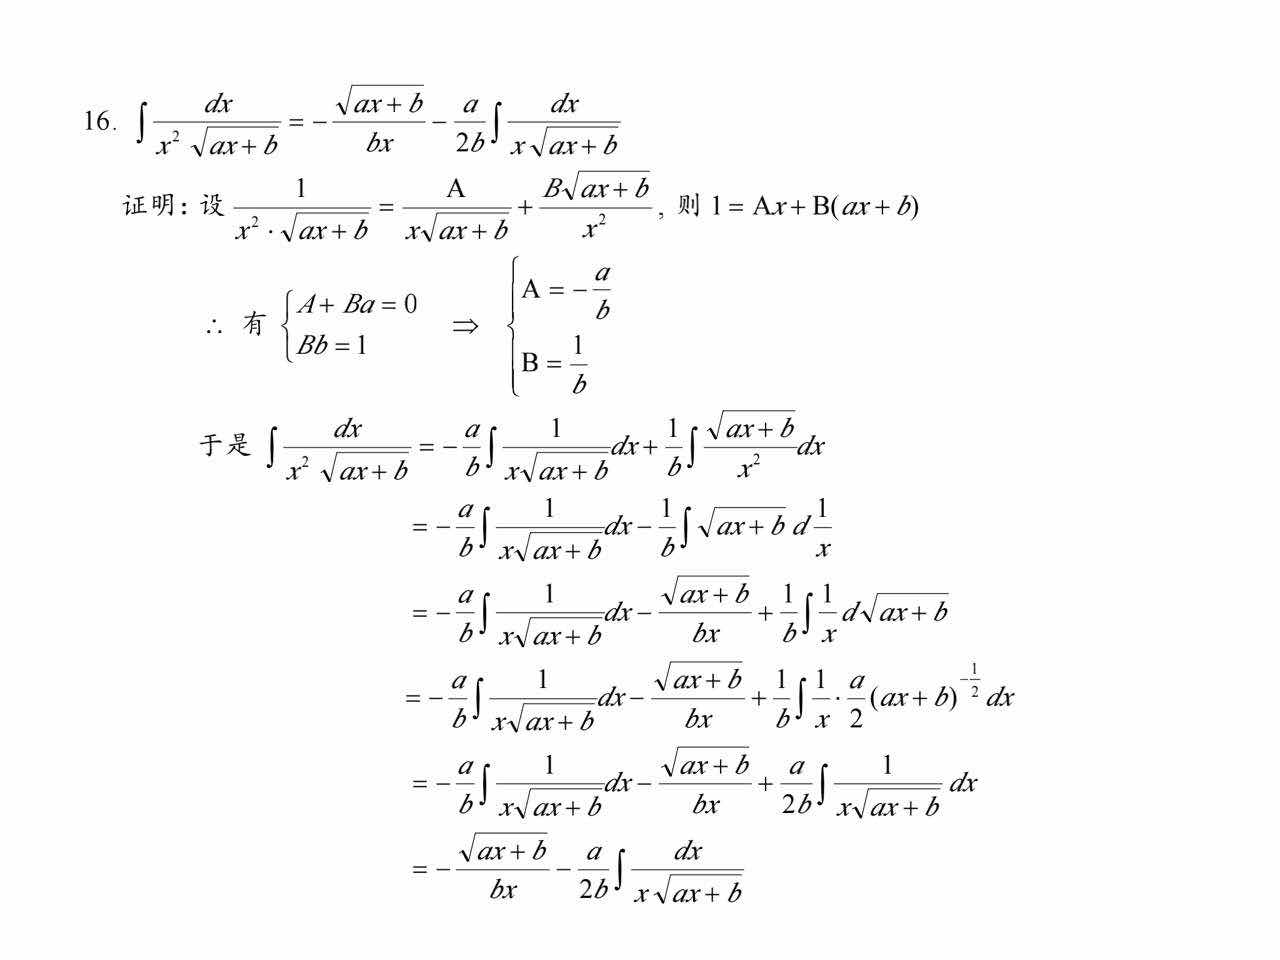
\includegraphics{./images/ch4/intExWHN.jpg}}
\end{center}